\documentclass[11pt]{article}
\usepackage[margin=1in]{geometry}
\usepackage{amsmath,amssymb,amsthm,mathtools,bm}
\usepackage{graphicx,booktabs,enumitem,xcolor}
\usepackage[round]{natbib}
\usepackage[colorlinks=true,linkcolor=violet,citecolor=violet,urlcolor=violet]{hyperref}
\newtheorem{theorem}{Theorem}[section]
\newtheorem{lemma}[theorem]{Lemma}
\newtheorem{proposition}[theorem]{Proposition}
\newtheorem{corollary}[theorem]{Corollary}
\theoremstyle{definition}
\newtheorem{definition}[theorem]{Definition}
\newtheorem{assumption}[theorem]{Assumption}
\theoremstyle{remark}
\newtheorem{remark}[theorem]{Remark}
\newcommand{\R}{\mathbb{R}}
\newcommand{\E}{\mathbb{E}}
\newcommand{\1}{\mathbf{1}}
\newcommand{\relu}{\mathrm{relu}}
\newcommand{\Lip}{\mathrm{Lip}}
\DeclareMathOperator*{\argmin}{arg\,min}
\title{Why Fault Detectors Learn the Wrong Rule:\\ Conjunctive Signatures, Composite Nulls, and the Supervision They Need\\[4pt]
\large Theory notes with complete proofs and numerical checks (draft)}
\author{Chirag Seth \quad University of Waterloo}
\date{October 2026}

\begin{document}
\maketitle

\begin{abstract}
A detector trained on normal versus one fault reaches near-perfect detection, yet in a fleet it flags many units that have a different fault or none. We model a multi-sensor fault as a \emph{conjunction}: $k$ signature channels shift together, at the same time. We prove five things.
(i) In the overlapping-class regime the detector that is optimal for the training task is \emph{additive} across channels, does not depend on class prevalence, and is what every cross-entropy-consistent learner converges to; more data converges \emph{to} the shortcut.
(ii) Its false-alarm rate on any partially overlapping fault follows a closed-form law that depends only on the target's detectability and the share of its signal the other fault reproduces. A corollary gives a \emph{detectability paradox}: the more reliably the target is detected, the more surely every partial look-alike is flagged. The resulting trade-off curve predicts the partial-match rates of the toy study's MLP and LSTM from their detection rate alone (0.72 vs.\ 0.73; 0.19 vs.\ 0.19–0.20).
(iii) Deployment is a test against a \emph{composite} null (normal or any fault that moves a strict subset of the signature). There, additive detectors lose a $\sqrt{k}$ factor in effective signal, or all power when overlap is unbounded; an intersection–union (``capped evidence'') detector is valid and within a factor $k$ of minimax.
(iv) In the separated regime the choice is made by implicit bias: any norm-bounded network places near-misses at least $1-\kappa/\sqrt{k}$ of the way from normal to fault, and rejecting all $k$ near-misses costs at least $k$ times the minimum path norm. This yields a necessary fraction of near-miss examples that grows with weight decay, roughly linearly for small weight decay.
(v) The minimal supervision that identifies the rule is $k$ channel near-misses plus $\binom{k}{2}$ temporal near-misses. The temporal count follows from Helly's theorem on the line, and it implies that fully staggered negatives teach nothing about simultaneity. All claims are checked numerically (Section~\ref{sec:checks}).
\end{abstract}

\tableofcontents
\newpage

%=====================================================================
\section{Results at a glance}
\begin{center}
\small
\begin{tabular}{p{4.3cm}p{6.2cm}p{4.2cm}}
\toprule
Result & Statement (informal) & Checked by \\
\midrule
Thm \ref{thm:np} & Training-optimal detector is additive; prevalence- and $n$-invariant; consistent learners converge to it & C1 (law holds for $n\ge 2000$, all prevalences) \\
Thm \ref{thm:law}, Cor \ref{cor:paradox} & Partial-overlap false-alarm law; power--specificity curve; detectability paradox & C1, C2, C8 (toy slide 12) \\
Thm \ref{thm:composite}, Prop \ref{prop:cap} & Composite null: additive loses $\sqrt{k}$ or everything; intersection--union near-minimax; capped evidence is necessary & C3 \\
Thm \ref{thm:ratio}, \ref{thm:pathnorm} & Near-miss position $\ge 1-\kappa\rho$; rejecting near-misses costs $\ge k\cdot$ path norm & C4 \\
Prop \ref{prop:pstar} & Necessary near-miss fraction $p^*(\lambda)$, increasing in $\lambda$ & C9, C5 \\
Lemma \ref{lem:blind}, \ref{lem:sign} & Window statistics are blind to timing and to sign & C6a \\
Lemma \ref{lem:ar} & Temporal dependence enters only through $\sigma_{\rm eff}$ & C7 \\
Thm \ref{thm:teach}, \ref{thm:helly} & Minimal teaching set: $k$ channel + $\binom{k}{2}$ temporal near-misses & C6b \\
Prop \ref{prop:samples} & How many examples per near-miss type & --- \\
\bottomrule
\end{tabular}
\end{center}

\paragraph{Corrections to earlier slides.} (1) ``Adding per-sensor evidence cannot express the AND'' is true only for \emph{uncapped} evidence; a generalized additive model with bounded per-channel terms can represent it (Prop.~\ref{prop:cap}). (2) The $\delta/(2\sqrt{k})$ margin statement applies to \emph{linear} additive detectors.

%=====================================================================
\section{Setting}\label{sec:setting}
A window is $X\in\R^{T\times C}$ ($T$ time steps, $C$ channels). Normal windows are $X=W$ with $W$ a stationary noise process. The target fault has signature $S\subseteq[C]$, $|S|=k\ge 2$, directions $s_j\in\{\pm1\}$, magnitudes $\delta_j>0$ and an active interval $I\subseteq[T]$:
\[
X = W + \textstyle\sum_{j\in S} s_j\delta_j\,\1_I\, e_j^\top .
\]
\paragraph{Shift statistic.} For a baseline set $B\subset[T]$ disjoint from $I$, let
$a_j(X)=s_j\big(\tfrac{1}{|I|}\sum_{t\in I}X_{tj}-\tfrac{1}{|B|}\sum_{t\in B}X_{tj}\big)$ (with $s_j=+1$ for $j\notin S$).
\begin{assumption}[Gaussian shift]\label{ass:gauss}
$W$ is a stationary Gaussian process. Then $a\sim N(0,\Sigma)$ under normal and $a\sim N(\bm\delta,\Sigma)$ under the target, with $\bm\delta=(\delta_j\1[j\in S])_j$ and $\Sigma$ determined by the autocovariance of $W$ (Lemma~\ref{lem:ar}).
\end{assumption}
Sections~\ref{sec:overlap}--\ref{sec:composite} work with $a$ (the onset is treated as known); Sections~\ref{sec:separated}--\ref{sec:supervision} also cover raw windows.

\paragraph{Other faults.} A fault with shift vector $\mu$ produces $a\sim N(\mu,\Sigma)$. Special cases: the $m$-of-$k$ \emph{partial} fault $\mu=\bm\delta\odot\1_{S'}$ with $S'\subset S$, $|S'|=m$; the \emph{near-miss} $m=k-1$; \emph{BIG} $\mu=c\,\delta_je_j$; \emph{flip} $\mu=-\bm\delta$; \emph{off-signature} $\mu$ supported on $S^c$.

\paragraph{Notation.} $\Phi$ is the standard normal CDF, $z_\alpha=\Phi^{-1}(1-\alpha)$, $D^2=\bm\delta^\top\Sigma^{-1}\bm\delta$ (target detectability), and
\[
r(\mu)=\frac{\bm\delta^\top\Sigma^{-1}\mu}{D^2}\qquad\text{(share of the target's signal that $\mu$ reproduces).}
\]
A detector is \emph{$\alpha$-calibrated} if it flags a fraction $\alpha$ of normal windows (as in all experiments).

%=====================================================================
\section{Regime I (overlapping classes): the shortcut is optimal for the training task}\label{sec:overlap}

\begin{theorem}[Training-optimal detector]\label{thm:np}
Under Assumption~\ref{ass:gauss}, let the training prevalence of the target be $\pi\in(0,1)$.
\begin{enumerate}[label=(\roman*)]
\item The Bayes log-odds is $\ell_\pi(a)=\bm\delta^\top\Sigma^{-1}a-\tfrac12D^2+\log\tfrac{\pi}{1-\pi}$, which is additive (linear) in $a$.
\item For every $\alpha\in(0,1)$ the most powerful size-$\alpha$ test of normal against target is $\phi^*(a)=\1\{\bm\delta^\top\Sigma^{-1}a>z_\alpha D\}$. It does not depend on $\pi$.
\item Let $\hat f_n$ be any learner with $\hat f_n\to\ell_\pi$ in probability under the training mixture $P_\pi=(1-\pi)N(0,\Sigma)+\pi N(\bm\delta,\Sigma)$. This includes gradient-descent logistic regression, whose model is well specified by (i), and any cross-entropy-consistent flexible learner. Let $\hat\phi_n=\1\{\hat f_n>\hat t_n\}$ with $\hat t_n$ the $(1-\alpha)$-quantile of $\hat f_n$ under $N(0,\Sigma)$. Then for every distribution $Q$ absolutely continuous with respect to Lebesgue measure, $Q(\hat\phi_n\ne\phi^*)\to0$.
\end{enumerate}
\end{theorem}
\begin{proof}
(i) The ratio of the two Gaussian densities with common covariance is $\exp(\bm\delta^\top\Sigma^{-1}a-\frac12\bm\delta^\top\Sigma^{-1}\bm\delta)$. Bayes' rule adds $\log\frac{\pi}{1-\pi}$.

(ii) By the Neyman--Pearson lemma, the most powerful test rejects for large likelihood ratio, which is increasing in $u=\bm\delta^\top\Sigma^{-1}a$. Under the null $u\sim N(0,D^2)$, so the size-$\alpha$ threshold is $z_\alpha D$. The prior does not appear.

(iii) Write $t^*$ for the $(1-\alpha)$-quantile of $\ell_\pi$ under $P_0=N(0,\Sigma)$; then $\{\ell_\pi>t^*\}=\{\phi^*=1\}$ by (ii). Since $P_0\le P_\pi/(1-\pi)$, convergence in $P_\pi$-probability implies convergence in $P_0$-probability. Under $P_0$, $\ell_\pi$ is Gaussian with a continuous, strictly increasing CDF, so the quantiles converge: $\hat t_n\to t^*$. Fix $\varepsilon>0$. The disagreement set is contained in
\[
\{|\ell_\pi-t^*|\le2\varepsilon\}\ \cup\ \{|\hat f_n-\ell_\pi|>\varepsilon\}\ \cup\ \{|\hat t_n-t^*|>\varepsilon\}.
\]
The third event is deterministic and eventually empty. $Q$ is absolutely continuous and $P_\pi$ has an everywhere-positive density, so $Q\ll P_\pi$. For a finite measure this gives, for every $\eta>0$, a $\gamma>0$ with $P_\pi(A)<\gamma\Rightarrow Q(A)<\eta$; hence $Q(|\hat f_n-\ell_\pi|>\varepsilon)\to0$. Finally $Q(|\ell_\pi-t^*|\le2\varepsilon)\to0$ as $\varepsilon\to0$, because $\ell_\pi$ is a non-degenerate affine function of $a$ and so has no atom under $Q$.
\end{proof}

\begin{remark}[Interpretation]
In this regime the ``broad'' rule is not a learning failure. It is the unique optimum of the training problem, and more data, rebalancing or longer training make a learner converge to it. Theorem~\ref{thm:np} extends to exponential-family noise with channel-separable sufficient statistics: the log-odds is still additive in the sufficient statistics.
\end{remark}

\begin{theorem}[Partial-overlap false-alarm law]\label{thm:law}
Under Assumption~\ref{ass:gauss}, the training-optimal detector $\phi^*$ flags a fault with shift $\mu$ with probability
\[
\Pr_\mu(\phi^*=1)=\Phi\big(D\,r(\mu)-z_\alpha\big).
\]
In particular, with independent signature channels of equal noise $\sigma$ and equal shifts $\delta$ ($D=\delta\sqrt{k}/\sigma$):
\begin{gather*}
\text{$m$-of-$k$ partial: }\Phi\Big(\tfrac{m\delta}{\sigma\sqrt k}-z_\alpha\Big),\qquad
\text{BIG ($c\delta$ on one channel): }\Phi\Big(\tfrac{c\delta}{\sigma\sqrt k}-z_\alpha\Big),\\
\text{flip: }\Phi(-D-z_\alpha),\qquad
\text{off-signature: }\alpha .
\end{gather*}
\end{theorem}
\begin{proof}
Under $N(\mu,\Sigma)$ the statistic $u=\bm\delta^\top\Sigma^{-1}a$ is Gaussian with mean $\bm\delta^\top\Sigma^{-1}\mu=D^2r(\mu)$ and variance $\bm\delta^\top\Sigma^{-1}\Sigma\Sigma^{-1}\bm\delta=D^2$. Hence $\Pr(u>z_\alpha D)=\Phi(Dr(\mu)-z_\alpha)$. The special cases follow from $r=m/k$, $c/k$, $-1$ and $0$.
\end{proof}

\begin{corollary}[Power--specificity curve and the detectability paradox]\label{cor:paradox}
Let $\beta=\Phi(D-z_\alpha)$ be the detection rate of $\phi^*$. Then for every $\mu$
\[
\Pr_\mu(\phi^*=1)=\Phi\Big(r(\mu)\big(\Phi^{-1}(\beta)+z_\alpha\big)-z_\alpha\Big).
\]
For every partial fault with $r(\mu)\in(0,1)$ this is strictly increasing in $\beta$ and tends to $1$ as $\beta\to1$. Any change that makes the target easier to detect at a fixed false-alarm budget therefore increases false alarms on \emph{every} partially overlapping fault: larger shifts, less noise, longer windows, or weaker temporal correlation (Lemma~\ref{lem:ar}).
\end{corollary}
\begin{proof}
Substitute $D=\Phi^{-1}(\beta)+z_\alpha$ into Theorem~\ref{thm:law}. Monotonicity holds because $r>0$ and $\Phi$ is increasing.
\end{proof}

\begin{corollary}[Loudest-channel dominance]\label{cor:loud}
With independent channels, a fault that reproduces only channel $j$ is flagged with probability $\Phi(D r_j-z_\alpha)$, where $r_j=(\delta_j/\sigma_j)^2/D^2$ is channel $j$'s share of the target SNR. Faults that hit the loudest signature channel are flagged most; the near-miss that drops the loudest channel is flagged least.
\end{corollary}

\begin{remark}[Model-agnostic prediction]
If a trained model's score is close to an increasing function of the additive statistic, Corollary~\ref{cor:paradox} predicts its partial-match rate from its own detection rate, with no fitting. On the toy study (check C8) this gives P2 $0.72$ vs.\ $0.73$ and P1 $0.19$ vs.\ $0.19$--$0.20$ for the MLP and LSTM. Window-statistics models exceed the curve (P2 $0.83$--$0.89$ vs.\ $0.78$), consistent with their additional timing blindness (Lemma~\ref{lem:blind}).
\end{remark}
\begin{figure}[t]\centering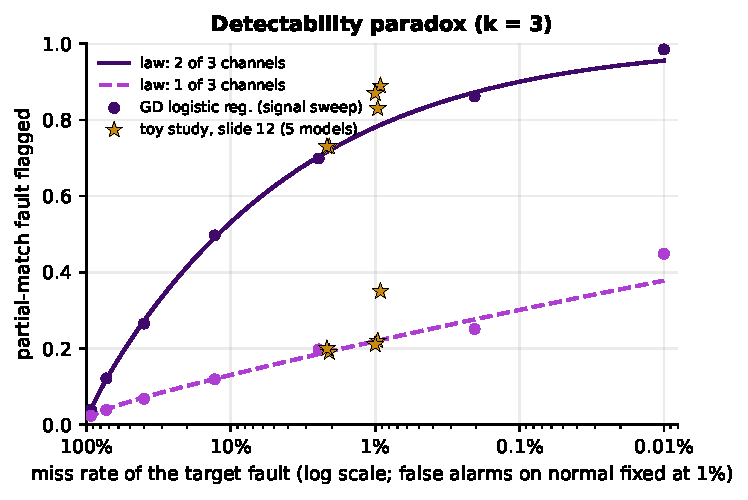
\includegraphics[width=0.58\linewidth]{figs/fig_tradeoff.pdf}
\caption{Power--specificity curve (Corollary~\ref{cor:paradox}), $k=3$, 1\% false alarms on normal. Lines: the law, no fitted parameters. Circles: gradient-descent logistic regression over a signal-strength sweep (check C2). Stars: the five models of the toy study at their own detection rates (check C8).}\label{fig:tradeoff}\end{figure}


\begin{remark}[Unknown onset]
Without an oracle onset, the likelihood-ratio detector scans candidate onsets, $\max_\tau \bm\delta^\top\Sigma^{-1}a(\tau)$. It is still additive across channels at every $\tau$, so partial faults with $r>0$ raise every scanned statistic. The exact law becomes a scan-statistic tail and is left open (Section~\ref{sec:open}).
\end{remark}

%=====================================================================
\section{What deployment needs: a composite null}\label{sec:composite}
In a fleet, ``not the target'' means normal \emph{or} any other fault. The faults that matter move a strict subset of the signature. Take independent signature channels with noise $\sigma_j$, detectors that depend on $a_S$ only, and fault-direction shifts. Define the \emph{overlap null}
\[
\mathcal N_{k-1}(M)=\big\{N(\mu,\Sigma):\ \operatorname{supp}(\mu)\subseteq S'\subsetneq S,\ 0\le\mu_j\le M_j\big\},\qquad M\in(0,\infty]^k .
\]
A detector is \emph{deployment-valid} at level $\alpha$ if $\sup_{Q\in\{P_0\}\cup\mathcal N_{k-1}(M)}Q(\phi=1)\le\alpha$.

\begin{theorem}[Composite null]\label{thm:composite}
Let $M_j\ge\delta_j$ for all $j$.
\begin{enumerate}[label=(\alph*)]
\item \emph{(Upper bound.)} Every deployment-valid level-$\alpha$ test has target power at most $\min_{j\in S}\Phi(\delta_j/\sigma_j-z_\alpha)$.
\item \emph{(Intersection--union attains it up to a factor $k$.)} $\phi_{IU}(a)=\1\{\min_{j\in S}a_j/\sigma_j>z_\alpha\}$ is deployment-valid for $M=\infty$. Its power is $\prod_{j}\Phi(\delta_j/\sigma_j-z_\alpha)$, so its miss probability is at most $\sum_j\Phi(z_\alpha-\delta_j/\sigma_j)\le k\cdot\max_j\Phi(z_\alpha-\delta_j/\sigma_j)$, i.e.\ at most $k$ times the minimax lower bound on the miss probability from (a).
\item \emph{(Additive, bounded overlap.)} With equal $\delta,\sigma$ and $M=\delta$, every deployment-valid linear detector $\1\{w^\top a_S>t\}$ with $w\ge0$ has power at most $\Phi(\delta/(\sigma\sqrt k)-z_\alpha)$, with equality at $w=\1$.
\item \emph{(Additive, unbounded overlap.)} If $M=\infty$, every deployment-valid linear detector with $w\ge0$, $w\ne0$ has power $0$.
\item \emph{(What training produces.)} The training-optimal detector $\phi^*$ is not deployment-valid: its false-alarm rate on the worst near-miss is $\Phi\big((k-1)\delta/(\sigma\sqrt k)-z_\alpha\big)>\alpha$ (equal case).
\end{enumerate}
\end{theorem}
\begin{proof}
(a) Fix $j$ and let $\mu^{(j)}=\bm\delta-\delta_je_j\in\mathcal N_{k-1}(M)$. A deployment-valid $\phi$ is in particular a level-$\alpha$ test of $N(\mu^{(j)},\Sigma)$ against $N(\bm\delta,\Sigma)$. These two laws differ only in the mean of coordinate $j$, by $\delta_j$, so by Neyman--Pearson the most powerful level-$\alpha$ test has power $\Phi(\delta_j/\sigma_j-z_\alpha)$. Take the minimum over $j$.

(b) Size (Berger, 1982): for $Q\in\mathcal N_{k-1}(\infty)$ some $j\in S\setminus S'$ has $\mu_j=0$, so $Q(\phi_{IU}=1)\le Q(a_j>z_\alpha\sigma_j)=\alpha$. Under $P_0$ the same bound holds. Power: the channels are independent and each event $\{a_j>z_\alpha\sigma_j\}$ has probability $\Phi(\delta_j/\sigma_j-z_\alpha)$ under the target. The miss bound follows from $1-\prod_j(1-x_j)\le\sum_jx_j$.

(c) Write $\|w\|=\|w\|_2$. Validity on $\mu=\delta(\1-e_i)$ for each $i$ requires $t\ge\delta\sum_{j\ne i}w_j+z_\alpha\sigma\|w\|$. The binding constraint is $i=\arg\min_jw_j$, so $t\ge\delta(\|w\|_1-\min_jw_j)+z_\alpha\sigma\|w\|$. The power is $\Phi\big((\delta\|w\|_1-t)/(\sigma\|w\|)\big)\le\Phi\big(\delta\min_jw_j/(\sigma\|w\|)-z_\alpha\big)$. Finally $\min_jw_j\le\|w\|/\sqrt k$, with equality iff $w\propto\1$.

(d) Pick $j$ with $w_j>0$. Since $k\ge2$, some $S'\ni j$ with $|S'|=k-1$ exists, so $\mu=Ae_j\in\mathcal N_{k-1}(\infty)$ for every $A>0$. Under $N(\mu,\Sigma)$, $w^\top a_S\sim N(w_jA,\sigma^2\|w\|^2)$, so the false-alarm rate tends to $1$ as $A\to\infty$ for any finite $t$. Validity forces $t=+\infty$, hence zero power.

(e) Theorem~\ref{thm:law} with $r=(k-1)/k$.
\end{proof}

\begin{proposition}[Capped evidence is necessary and sufficient]\label{prop:cap}
Consider generalized additive detectors $\1\{\sum_{j\in S}g_j(a_j)>t\}$ with nondecreasing $g_j$, under $M=\infty$.
\begin{enumerate}[label=(\alph*)]
\item If some $g_j$ is unbounded above, every deployment-valid such detector has power $0$.
\item If every $g_j$ is bounded, the class contains $\phi_{IU}$ (take $g_j=\1\{a_j>z_\alpha\sigma_j\}$ and $t=k-\frac12$), so it attains Theorem~\ref{thm:composite}(b).
\end{enumerate}
The same holds for channel-independent sequence models $f(X)=\sum_jh_j(X_{\cdot j})$, the structure of per-channel encoders with a linear head: such a model is deployment-valid with nontrivial power only if each $h_j$ is bounded along fault-direction shifts.
\end{proposition}
\begin{proof}
(a) Repeat the proof of Theorem~\ref{thm:composite}(d) with $g_j(a_j)\to\infty$ in place of $w_ja_j\to\infty$. The other summands are fixed in distribution, so the false-alarm rate tends to $1$ for any finite $t$.
(b) is the construction stated. For the sequence-model version, apply (a) to $h_j$ evaluated along $X+A\,s_j\1_Ie_j^\top$, $A\to\infty$.
\end{proof}

\begin{figure}[t]\centering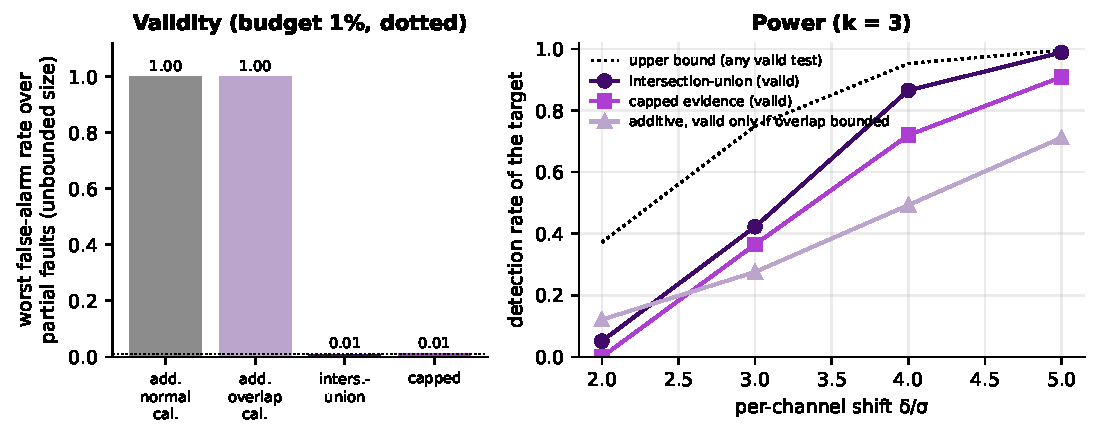
\includegraphics[width=0.9\linewidth]{figs/fig_composite.pdf}
\caption{Composite null, $k=3$ (check C3). Left: worst false-alarm rate over partial faults of unbounded size. Detectors that add uncapped evidence are invalid. Right: target detection rate of the valid detectors and of the additive detector that is valid only when overlaps are bounded by the target's own shift.}\label{fig:composite}\end{figure}
\begin{remark}
Proposition~\ref{prop:cap} replaces the earlier slide statement. The channel-independent model in our experiments uses ReLU encoders with a linear head and is unbounded; it flags one-loud-channel faults at $0.99$--$1.00$ and stays at $0.67$ on near-misses after the fix. The theory predicts that a \emph{capped} version (bounded per-channel output) can be fixed. This is now an experiment in the pipeline.
\end{remark}

%=====================================================================
\section{Regime II (separated classes): what gradient descent picks}\label{sec:separated}
When normal and fault are well separated (our real-data targets: one sensor alone gives 89--99.8\% training accuracy), near-misses have negligible training density and Theorem~\ref{thm:np}(iii) no longer pins down the detector there. Many rules fit the training data. Gradient descent on homogeneous networks with logistic loss converges in direction to a KKT point of the minimum-norm (maximum-margin) problem \citep{lyu2020,ji2020}, and weight decay explicitly penalises the norm. Both favour small norm, and small norm bounds the Lipschitz constant.

\begin{lemma}[Norm bounds Lipschitz]\label{lem:lip}
For $f(x)=\sum_iv_i\,\sigma(w_i^\top x+b_i)+c$ with $\sigma$ 1-Lipschitz, $|f(x)-f(y)|\le R(\theta)\|x-y\|$ with path norm $R(\theta)=\sum_i|v_i|\|w_i\|$. Moreover $\min_{\text{rescalings}}\tfrac12\sum_i(v_i^2+\|w_i\|^2+b_i^2)\ge R(\theta)$.
For depth-$L$ networks, $\Lip(f)\le\prod_l\|W_l\|_{op}\le(\|\theta\|^2/L)^{L/2}$.
\end{lemma}
\begin{proof}
$|f(x)-f(y)|\le\sum_i|v_i||w_i^\top(x-y)|\le\sum_i|v_i|\|w_i\|\|x-y\|$. For the second claim, $(v,w,b)\mapsto(v/\gamma,\gamma w,\gamma b)$ leaves $f$ unchanged, and $\min_\gamma\frac12(v^2/\gamma^2+\gamma^2(\|w\|^2+b^2))=|v|\sqrt{\|w\|^2+b^2}\ge|v|\|w\|$. The deep case is submultiplicativity followed by AM--GM.
\end{proof}

\begin{theorem}[Near-miss position]\label{thm:ratio}
Let $x_0,x_+$ be normal and fault prototypes with $\Delta=\|x_+-x_0\|$, and let $f$ satisfy $f(x_+)-f(x_0)=G>0$. Let $R_{\min}=G/\Delta$, the smallest Lipschitz constant compatible with this separation, which a single unit attains, and let $\kappa=\Lip(f)/R_{\min}\ge1$. For any $x$ with $\|x-x_+\|=\rho\Delta$,
\[
p(x):=\frac{f(x)-f(x_0)}{f(x_+)-f(x_0)}\ \ge\ 1-\kappa\rho .
\]
\end{theorem}
\begin{proof}
$f(x)\ge f(x_+)-\Lip(f)\rho\Delta=f(x_+)-\kappa\rho G$. Subtract $f(x_0)$ and divide by $G$.
\end{proof}

\begin{corollary}[Channel and temporal near-misses]\label{cor:nm}
\begin{enumerate}[label=(\alph*)]
\item In shift-statistic space with equal shifts, a channel near-miss has $\rho=1/\sqrt k$, so $p\ge1-\kappa/\sqrt k$. In raw windows where each signature channel is shifted by $\delta$ on $L$ steps, $\rho$ is again $\sqrt{L}\delta/(\sqrt{kL}\delta)=1/\sqrt k$.
\item A temporal near-miss that displaces one channel's shift block by $\Delta t\le L$ steps has $\|x-x_+\|=\delta\sqrt{2\Delta t}$, so $\rho=\sqrt{2\Delta t/(kL)}$ and $p\ge1-\kappa\sqrt{2\Delta t/(kL)}$. A low-norm detector cannot separate the target from a staggering of fewer than about $kL/(8\kappa^2)$ steps.
\end{enumerate}
An $\alpha$-calibrated threshold sits near the normal prototype, at some $p_\alpha$ small when noise is small. Any near-miss with $p(x)>p_\alpha$ is flagged.
\end{corollary}

\begin{theorem}[The narrow rule costs $k$ times the norm]\label{thm:pathnorm}
Let $f$ be a two-layer network as in Lemma~\ref{lem:lip} with ReLU activation, and let $x^{(j)}=x_+-\delta\,\1_{\mathcal B}e_j^\top$ be the channel-$j$ near-miss, where $\mathcal B$ is the shift block of length $L$ ($L=1$ in shift-statistic space). If $f(x_+)-f(x^{(j)})\ge g>0$ for every $j\in S$, then
\[
R(\theta)\ \ge\ \frac{\sqrt k\,g}{\delta\sqrt L},\qquad\text{so}\qquad\frac{R(\theta)}{R_{\min}}\ \ge\ k\,\frac{g}{G}.
\]
For unequal shifts, $R(\theta)\ge g\sum_{j\in S}\delta_j^{-1}/\sqrt{kL}$.
\end{theorem}
\begin{proof}
ReLU is 1-Lipschitz, so for each unit $|\relu(w_i^\top x_++b_i)-\relu(w_i^\top x^{(j)}+b_i)|\le\delta\sum_{t\in\mathcal B}|w_{i,tj}|$. Hence $g\le\delta\sum_i|v_i|\sum_{t\in\mathcal B}|w_{i,tj}|$ for each $j$. Summing over $j\in S$ and applying Cauchy--Schwarz to the $kL$ coordinates in $\mathcal B\times S$,
\[
kg\ \le\ \delta\sum_i|v_i|\,\|w_{i,\mathcal B\times S}\|_1\ \le\ \delta\sqrt{kL}\sum_i|v_i|\|w_i\|=\delta\sqrt{kL}\,R(\theta).
\]
Since $R_{\min}=G/\Delta=G/(\delta\sqrt{kL})$, the ratio follows. The unequal case replaces $kg\le\dots$ by $\sum_jg/\delta_j\le\dots$.
\end{proof}

Rejecting the near-misses down to the normal level ($g=G$) costs at least $k$ times the minimum path norm; pushing them to the midpoint ($g=G/2$) costs at least $k/2$. Check C4 measures ratios of $2.96$--$7.54$ for $k=2,\dots,8$ when near-misses are added (Figure~\ref{fig:separated}).
\begin{figure}[t]\centering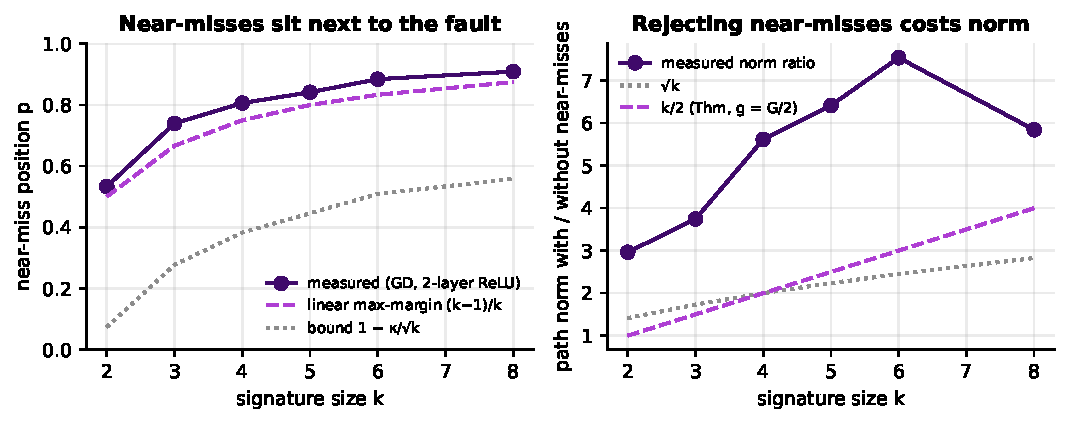
\includegraphics[width=0.9\linewidth]{figs/fig_separated.pdf}
\caption{Separated regime, two-layer ReLU networks trained by gradient descent (check C4). Left: where the near-miss lands between normal ($0$) and fault ($1$). Right: path-norm increase needed once near-misses are added as negatives.}\label{fig:separated}\end{figure}


\begin{proposition}[Exact linear limit under symmetric data; from \citet{lyu2021}]\label{prop:lyu}
If the training set is linearly separable and symmetric, i.e.\ closed under $(x,y)\mapsto(-x,-y)$ (true in distribution after centring balanced normal/fault data with symmetric noise; exactly after symmetrising the sample), then gradient flow from small initialisation on two-layer leaky-ReLU networks converges in direction to the linear max-margin classifier \citep[main theorem]{lyu2021}. For our prototypes that classifier is $w\propto\1_S$, so near-misses sit at exactly $p=(k-1)/k$. They are classified positive by the max-margin threshold for every $k\ge3$ and lie on it for $k=2$.
\end{proposition}

\begin{proposition}[How many near-misses beat weight decay]\label{prop:pstar}
Consider noise-free prototypes with masses $q$ at $x_0$ (label $-1$), $q$ at $x_+$ (label $+1$) and $p/k$ at each near-miss (label $-1$), $2q+p=1$, in shift-statistic space with equal shifts $\delta$. The objective is $J(\theta)=\sum\text{mass}\cdot\log(1+e^{-yf_\theta(x)})+\lambda R(\theta)$, the function-space form of $\ell_2$ weight decay by Lemma~\ref{lem:lip}. Define
\begin{align*}
J_{\rm cheap}(p)&=\min_{m_0,m_1\ge0}\ q\ell(m_0)+q\ell(m_1)+p\,\ell\!\Big(-m_1+\tfrac{m_0+m_1}{k}\Big)+\lambda\tfrac{m_0+m_1}{\delta\sqrt k},\\
B(p)&=\inf_{m,m_0\in\R}\ q\ell(m)+q\ell(m_0)+\lambda\max\Big(\tfrac{\sqrt k\,m_+}{\delta},\tfrac{|m+m_0|}{\delta\sqrt k}\Big),
\end{align*}
with $\ell(z)=\log(1+e^{-z})$. If $J_{\rm cheap}(p)<B(p)$, then every minimiser of $J$ flags at least one near-miss ($f(x^{(j)})>0$). Hence the near-miss fraction must exceed $p^*(\lambda,k)=\sup\{p:J_{\rm cheap}(p)<B(p)\}$ before weight-decay training can learn the narrow rule.
\end{proposition}
\begin{proof}
\emph{Upper bound.} The single unit $f(x)=v\,\relu(\1_S^\top x/\sqrt k)-m_0$ with $v=(m_0+m_1)/(\delta\sqrt k)$ satisfies $f(x_0)=-m_0$ and $f(x_+)=m_1$. It is linear along the prototypes, so $f(x^{(j)})=m_1-(m_0+m_1)/k$, and its path norm is $v$. Hence $\min J\le J_{\rm cheap}(p)$.

\emph{Lower bound.} Let $f$ reject every near-miss, $f(x^{(j)})\le0$, and set $m=f(x_+)$, $m_0=-f(x_0)$. The near-miss losses are nonnegative. Theorem~\ref{thm:pathnorm} with $g=m_+$ gives $R\ge\sqrt k\,m_+/\delta$, and Lemma~\ref{lem:lip} gives $R\ge|m+m_0|/(\delta\sqrt k)$. Hence $J(\theta)\ge B(p)$. If $J_{\rm cheap}(p)<B(p)$, no function rejecting all near-misses is a minimiser.
\end{proof}

Numerically (check C9, $\delta=1$): $p^*\approx0.0002$, $0.0013$, $0.0088$, $0.017$ for $\lambda=10^{-4},10^{-3},10^{-2},3\cdot10^{-2}$ at $k=3$, and $p^*$ grows with $k$ (Figure~\ref{fig:pstar}). The necessary fraction grows roughly linearly in $\lambda$ for small $\lambda$ and somewhat more slowly beyond. In finite-noise gradient-descent experiments (C5) the required amount is larger, and at $\lambda=10^{-2}$ even $128$ near-misses per type do not move the partial-match rate. This is a lower bound, not a sufficient condition.
\begin{figure}[t]\centering
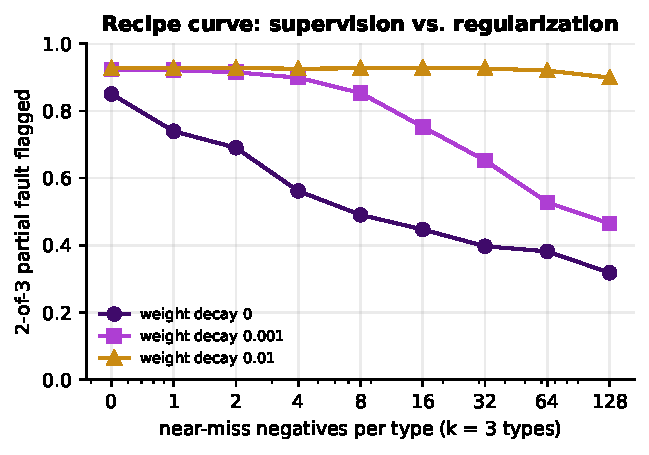
\includegraphics[width=0.48\linewidth]{figs/fig_recipe.pdf}\hfill
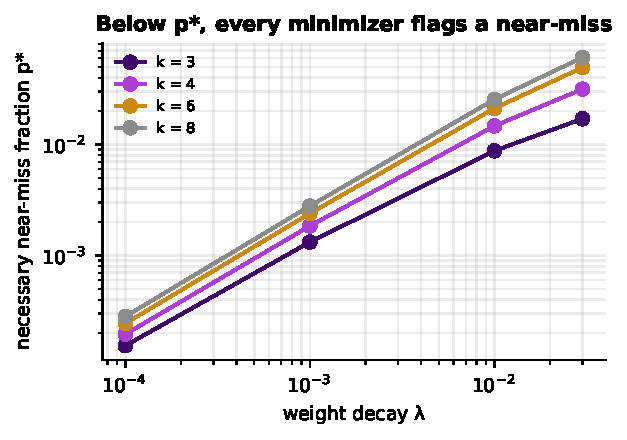
\includegraphics[width=0.46\linewidth]{figs/fig_pstar.pdf}
\caption{Left: partial-match false alarms vs.\ near-miss negatives per type, two-layer ReLU network trained by gradient descent with three weight decays (check C5). Right: the necessary near-miss fraction $p^*(\lambda,k)$ of Proposition~\ref{prop:pstar} (check C9).}\label{fig:recipe}\label{fig:pstar}
\end{figure}

%=====================================================================
\section{Time: what window features and temporal dependence do}\label{sec:time}
\begin{lemma}[Window statistics are timing-blind]\label{lem:blind}
Let $\psi:\R^T\to\R^q$ be invariant to permutations of the time index (mean, standard deviation, min, max, quantiles), and let $\Psi(X)=(\psi(X_{\cdot1}),\dots,\psi(X_{\cdot C}))$. Suppose the noise is exchangeable in time within each channel and independent across channels. If two shift patterns $G,G'\in\R^{T\times C}$ have, channel by channel, the same multiset of entries, then $\Psi(W+G)\overset{d}{=}\Psi(W+G')$. Every detector built on $\Psi$ flags simultaneous, staggered and pair-staggered faults with the same per-channel shift durations at identical rates.
\end{lemma}
\begin{proof}
For each $j$ choose a permutation $\pi_j$ of $[T]$ with $G'_{\cdot j}=G_{\pi_j(\cdot),j}$. Exchangeability gives $W_{\cdot j}\overset{d}{=}W_{\pi_j(\cdot),j}$, and independence across channels makes this hold jointly. Then $(W+G')_{\cdot j}\overset{d}{=}(W+G)_{\pi_j(\cdot),j}$ jointly over $j$, and $\psi$ is permutation-invariant.
\end{proof}
For AR noise or for statistics such as the slope and the last-8 mean, the invariance is approximate. This matches window-statistics models flagging staggered faults at $0.57$--$1.00$ on every target.

\begin{lemma}[Dispersion features are sign-blind]\label{lem:sign}
If $W\overset{d}{=}-W$ and $\psi$ is a dispersion functional ($\psi(-x)=\psi(x)$, e.g.\ standard deviation or range), then $\psi(W+G)\overset{d}{=}\psi(W-G)$. Detectors relying on dispersion flag a fault and its sign-flipped version equally.
\end{lemma}
\begin{proof}
$\psi(W+G)=\psi(-W-G)\overset{d}{=}\psi(W-G)$.
\end{proof}
This is consistent with the fan-coil LSTM flagging wrong-direction changes (0.46--0.83) and the toy gradient-boosting model's reliance on window standard deviation.

\begin{lemma}[Temporal dependence enters through $\sigma_{\rm eff}$]\label{lem:ar}
For stationary noise with autocovariance $\gamma(h)$, $\operatorname{Var}(a_j)=c^\top\Gamma c$ with $c=(-\1_B/|B|,\ \1_I/|I|)$ and $\Gamma_{st}=\gamma(s-t)$. For AR(1) with coefficient $\phi$ and marginal variance $\sigma_x^2$, the variance of an $L$-step mean is $\sigma_x^2L^{-2}\sum_{s,t}\phi^{|s-t|}\to\sigma_x^2(1+\phi)/((1-\phi)L)$. All results above hold with $\sigma\leftarrow\sigma_{\rm eff}$. A stickier process lowers $D$, which lowers both detection and partial false alarms along the same curve (Corollary~\ref{cor:paradox}). For sample sizes, $n$ consecutive windows count as $n_{\rm eff}=n(1-\phi)/(1+\phi)$.
\end{lemma}
\begin{proof}
$a_j$ is the linear functional $c^\top W_{\cdot j}$ plus a constant. The AR(1) limit is the standard series $\sum_{h\in\mathbb Z}\phi^{|h|}=(1+\phi)/(1-\phi)$. Check C7 matches the exact formula to within sampling error.
\end{proof}

%=====================================================================
\section{Minimal supervision: what to add and how much}\label{sec:supervision}
Normal-vs-fault data label only the bottom ($\bm0$) and top ($\1$) of the pattern lattice. For $k=3$, $18$ monotone rules fit those labels perfectly ($20$ monotone Boolean functions of three variables minus the two constants), and AND and OR are both among them.

\begin{theorem}[Channel teaching set]\label{thm:teach}
Let $\mathcal H=\{h:\{0,1\}^k\to\{0,1\}\ \text{monotone},\ h(\bm0)=0,\ h(\1)=1\}$. A set $\mathcal L\subseteq\{0,1\}^k$ labelled by AND identifies AND within $\mathcal H$ if and only if $\mathcal L\supseteq\{\1-e_j:j\in[k]\}$.
\end{theorem}
\begin{proof}
($\Leftarrow$) Any $x\ne\1$ has some $x_j=0$, so $x\le\1-e_j$, and monotonicity gives $h(x)\le h(\1-e_j)=0$.
($\Rightarrow$) If $\1-e_i\notin\mathcal L$, then $h_i(x)=\1\{x\ge\1-e_i\}$ is monotone with $h_i(\bm0)=0$ (as $k\ge2$) and $h_i(\1)=1$. It equals AND everywhere except at $\1-e_i$, so it is consistent with $\mathcal L$ and differs from AND.
\end{proof}
This is the standard boundary characterisation of teaching sets for monotone functions \citep{goldman1995}; it is included for completeness. The new part is the temporal analogue.

\begin{theorem}[Temporal teaching set via Helly]\label{thm:helly}
Let each signature channel be shifted on a nonempty interval $I_j\subseteq[0,T)$, and let $\mathcal G(I)$ be the overlap graph on $S$ (edge $ij$ iff $I_i\cap I_j\ne\emptyset$).
\begin{enumerate}[label=(\alph*)]
\item (Helly, $d=1$) $\bigcap_jI_j\ne\emptyset$ if and only if $\mathcal G(I)=K_k$.
\item Consider rules $h(I)=H(\mathcal G(I))$ with $H$ monotone under edge inclusion and $H(K_k)=1$. A labelled set identifies the simultaneity rule $H^*(G)=\1\{G=K_k\}$ within this class if and only if it contains, for every edge $e$, a negative with overlap graph $K_k-e$.
\item Each $K_k-e$ is realisable by intervals of equal length (so per-channel shift durations match the target's): for $e=\{a,b\}$ take $I_a=[0,1)$, $I_b=[1,2)$ and $I_j=[\tfrac12,\tfrac32)$ otherwise.
\item A fully staggered negative (empty overlap graph) is the bottom of the lattice. For $k\ge3$, labelling it $0$ does not identify $H^*$. (For $k=2$, $K_2-e$ \emph{is} the empty graph, so the two notions coincide.)
\end{enumerate}
\end{theorem}
\begin{proof}
(a) Pairwise-intersecting intervals have a common point: with $I_j=[l_j,u_j)$, pairwise intersection gives $\max_jl_j<\min_ju_j$, and any point in between is common. The converse is trivial.
(b) Identify $G$ with its edge-indicator vector in $\{0,1\}^{\binom k2}$. Then $H^*$ is the AND of the edge indicators. Sufficiency: every $G\ne K_k$ is contained in some $K_k-e$, so $H(G)\le H(K_k-e)=0$. Necessity: if $K_k-e$ is not labelled, $H_e(G)=\1\{G\supseteq K_k-e\}$ is monotone, satisfies $H_e(K_k)=1$, and differs from $H^*$ only at $K_k-e$. It is therefore consistent with every other labelled configuration.
(c) $I_a\cap I_j=[\tfrac12,1)$, $I_b\cap I_j=[1,\tfrac32)$, $I_j\cap I_{j'}=I_j$, and $I_a\cap I_b=\emptyset$. (d) For $k\ge3$, $K_k-e$ has at least two edges, so $H(G)=\1\{G\supseteq K_k-e\}$ is monotone, equals $0$ on the empty graph, and differs from $H^*$.
\end{proof}

\begin{corollary}[Total near-miss types]
A configuration is a pair $(A,G)$: the set $A\subseteq S$ of shifted signature channels and the overlap graph $G$ on $A$, ordered by $(A,G)\preceq(A',G')$ iff $A\subseteq A'$ and $G\subseteq G'$. The target rule is $\1\{A=S,\ G=K_k\}$. Within rules monotone in this order, identification requires and is achieved by the $k+\binom k2=k(k+1)/2$ maximal non-target configurations: $(S\setminus\{j\},K_{k-1})$ for each $j$ and $(S,K_k-e)$ for each edge $e$.
\end{corollary}
\begin{proof}
Every non-target $(A,G)$ has either $A\ne S$, and then $(A,G)\preceq(S\setminus\{j\},K_{k-1})$ for some $j\notin A$, or $A=S$ and $G\ne K_k$, and then $(A,G)\preceq(S,K_k-e)$ for a missing edge $e$. Sufficiency follows by monotonicity. Necessity is the argument of Theorems~\ref{thm:teach} and \ref{thm:helly}(b): the up-set indicator of an unlabelled maximal configuration is monotone and differs from the target only there.
\end{proof}

Check C6b confirms the prediction of Theorem~\ref{thm:helly}(d) with a raw-series network trained by gradient descent. Fully staggered negatives fix fully staggered faults ($0.96\to0.01$) but leave pair-staggered ones at $0.94$. Pair-staggered negatives fix both ($0.00$ and $0.16$). In our real-data pipeline the ``staggered negatives'' were fully staggered, which explains why they did not generalise; the pipeline now has pair-staggered negatives.
\begin{figure}[t]\centering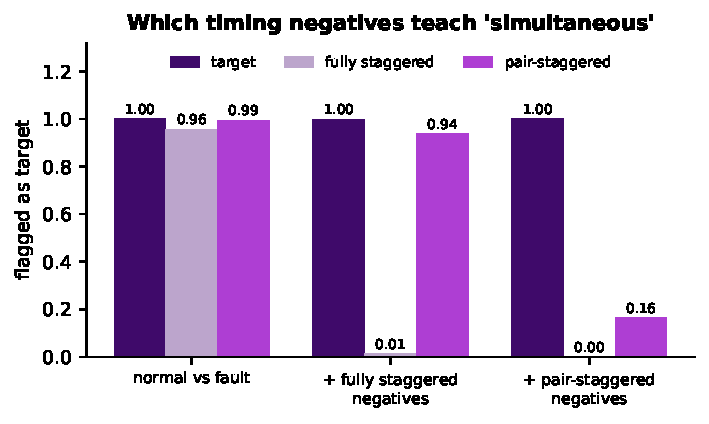
\includegraphics[width=0.6\linewidth]{figs/fig_helly.pdf}
\caption{Temporal teaching set (check C6b). A raw-series network trained only on normal vs.\ fault flags both staggered variants. Fully staggered negatives fix only fully staggered faults. Pair-staggered negatives (the Helly boundary) fix both.}\label{fig:helly}\end{figure}


\begin{proposition}[How many examples per near-miss type]\label{prop:samples}
For a learner with the intersection--union structure built in (per-channel thresholds, then AND), let channel $j$ have a level $\nu_j$ in its near-miss and $\nu_j+\Delta_j$ in the target, with noise $\sigma_j$ (effective, Lemma~\ref{lem:ar}). Set $\hat c_j$ to the midpoint of the sample means from $n$ near-misses of type $j$ and $n$ targets. If
\[
n\ \ge\ \frac{32\,\max_j\sigma_j^2}{\min_j\Delta_j^2}\,\log\frac{4k}{\eta},
\]
then with probability at least $1-\eta$, every threshold is within $\Delta_j/4$ of its midpoint. The learned rule then flags near-miss $j$ with probability at most $\Phi(-\Delta_j/(4\sigma_j))$ and misses the target with probability at most $\sum_j\Phi(-\Delta_j/(4\sigma_j))$. For windows drawn consecutively from an AR(1) process, replace $n$ by $n_{\rm eff}$.
\end{proposition}
\begin{proof}
A mean of $n$ independent $N(\mu,\sigma^2)$ samples deviates by more than $t$ with probability at most $2e^{-nt^2/(2\sigma^2)}$. The midpoint error is at most the larger of the two mean errors, so with $t=\Delta_j/4$ the failure probability for channel $j$ is at most $4e^{-n\Delta_j^2/(32\sigma_j^2)}$; a union bound over $j$ gives the condition. On success $\hat c_j\ge\nu_j+\Delta_j/4$, so near-miss $j$ exceeds it with probability at most $\Phi(-\Delta_j/(4\sigma_j))$; the target bound is symmetric plus a union bound. Under dependence the variance of the mean is inflated by $(1+\phi)/(1-\phi)$ (Lemma~\ref{lem:ar}).
\end{proof}
Using near-misses rather than normal data matters when sensors are coupled. In a real near-miss, channel $j$'s level $\nu_j$ is shaped by the other faulty channels and need not equal its normal level.

%=====================================================================
\section{Answer: why, what is missing, and the recipe}
\paragraph{Why.} In both regimes the detector learned from normal-vs-fault data is additive or Lipschitz-small across channels and time. With overlapping classes this is the Bayes-optimal training rule (Theorem~\ref{thm:np}) and gradient descent converges to it. With separated classes, implicit bias selects small-norm solutions, which cannot separate the target from near-misses without paying $k$ times the norm (Theorems~\ref{thm:ratio}--\ref{thm:pathnorm}). The narrow rule is never favoured, and the stronger the target, the worse the partial-match false alarms (Corollary~\ref{cor:paradox}).

\paragraph{What is missing.} Not data volume or class balance (Theorem~\ref{thm:np}(ii)--(iii)), but one of the following:
(1) the right null: calibrate against normal \emph{and} near-misses (Theorem~\ref{thm:composite});
(2) the right supervision: $k$ channel and $\binom k2$ temporal near-misses (Theorems~\ref{thm:teach}--\ref{thm:helly});
(3) the right inductive bias: capped per-channel evidence or an intersection--union structure (Proposition~\ref{prop:cap}).

\paragraph{Recipe.}
\begin{enumerate}[leftmargin=*]
\item Estimate the signature $S$ from fault vs.\ normal data (top-$k$ standardised shifts).
\item Either build the conjunction in (per-channel capped evidence, then AND) or train a flexible model with near-miss negatives of all $k+\binom k2$ types, using \emph{pair}-staggered rather than fully staggered timing negatives.
\item Amounts: structured learner, $n\ge32(\sigma_{\rm eff}/\Delta)^2\log(4k/\eta)$ per type (Proposition~\ref{prop:samples}). Black-box with weight decay $\lambda$, near-miss fraction above $p^*(\lambda,k)$, which grows with $\lambda$ (Proposition~\ref{prop:pstar}); in practice more (Figure~\ref{fig:recipe}).
\item Calibrate the alarm threshold so that near-misses, not only normal windows, stay below the budget.
\end{enumerate}

%=====================================================================
\section{Numerical checks}\label{sec:checks}
All checks are in \texttt{theory/theory\_checks.py} (NumPy and SciPy; gradient-descent learners where the claim is about gradient descent). Output is in \texttt{theory/checks\_out/}.
\begin{description}[leftmargin=1.2cm,style=nextline]
\item[C1] GD logistic regression, $k=3$, $\delta/\sigma=1.5$: predicted vs.\ measured range over $n\in\{2000,20000\}$ and prevalence $\in\{0.1,0.5,0.9\}$: CAP $0.607$ ($0.585$--$0.610$), P2 $0.276$ ($0.250$--$0.282$), P1 $0.072$ ($0.064$--$0.072$), BIG1 $0.607$ ($0.544$--$0.619$), UP $0.000$ ($0.000$), OFF $0.010$ ($0.008$--$0.012$). A two-layer network follows the trade-off curve from its own detection rate (P2 $0.208$ predicted vs.\ $0.203$).
\item[C2] Paradox: as $\delta/\sigma$ goes $0.5\to4$, measured P2 goes $0.039\to0.985$ (predicted $0.040\to0.989$).
\item[C3] Composite null: additive detectors calibrated on normal have size $0.49$--$1.00$ on near-misses; under unbounded overlap every additive detector has size $1.00$. The intersection--union detector has size $0.010$ and power $0.051/0.423/0.866/0.989$ at $\delta/\sigma=2/3/4/5$, matching $\Phi(\delta/\sigma-z)^3$; the bounded-null additive detector has $0.121/0.276/0.493/0.712$; the capped GAM is valid with power $0.00/0.37/0.72/0.91$ (Figure~\ref{fig:composite}).
\item[C4] Gradient-descent ReLU nets, separated classes: near-miss position $0.53$--$0.91$ ($\ge$ linear $(k-1)/k$ and $\ge$ the bound), $\kappa\approx1.2$--$1.3$, near-misses flagged $98$--$100\%$. Adding near-misses raises the normalised path norm by $2.96$--$7.54\times$ ($\ge\sqrt k$; Theorem~\ref{thm:pathnorm} gives $\ge k\,g/G$).
\item[C5] P2 false alarms vs.\ near-misses per type ($0\to128$): $0.85\to0.32$ without weight decay; $0.92\to0.46$ at $\lambda=10^{-3}$; flat at $0.93\to0.90$ at $\lambda=10^{-2}$.
\item[C6] (a) Window statistics (mean, sd, min, max) with i.i.d.\ noise: target, fully staggered and pair-staggered (equal durations) flagged at $0.276/0.274/0.270$, as Lemma~\ref{lem:blind} requires. (b) Helly: see Section~\ref{sec:supervision} and Figure~\ref{fig:helly}.
\item[C7] AR(1) variance formula vs.\ simulation: agreement within sampling error.
\item[C8] Toy slide 12 predicted from detection rate alone: MLP/LSTM P2 $0.72$ vs.\ $0.73$, P1 $0.19$ vs.\ $0.19$/$0.20$.
\item[C9] Necessary near-miss fraction $p^*(\lambda)$, as in Proposition~\ref{prop:pstar}.
\end{description}

\subsection*{Pipeline experiments on the toy replica (slide-7 data, LSTM and five other models)}
Same code path as the real-data runs (\texttt{run\_toy.py}, \texttt{reference\_results/toy\_theory}). Noisy, overlapping-class regime.
\begin{center}\small
\begin{tabular}{p{4.2cm}p{7.6cm}p{2.6cm}}
\toprule
Prediction & Toy result (LSTM unless stated) & Verdict \\
\midrule
Partial-match law (Cor.~\ref{cor:paradox}), from CAP + single-channel rates & P2 predicted $0.58$, measured $0.58$ & holds \\
Paradox: stronger fault $\Rightarrow$ more partial alarms & scale $\times0.25/0.5/0.75/1/1.5$: CAP $0.09/0.27/0.74/0.96/1.00$, P2 $0.05/0.10/0.34/0.59/0.94$; law $0.05/0.12/0.37/0.66/0.89$. Same pattern for all five models. & holds \\
Capped evidence ignores one loud channel (Prop.~\ref{prop:cap}) & BIG1 flagged, no fix: capped CI $0.08$ vs uncapped CI $0.99$ & holds \\
Capped CI is fixable, uncapped is not & after all-but-one negatives P2: capped $0.37\to0.22$, uncapped $0.72\to0.35$ & partial \\
Recipe: more near-misses $\Rightarrow$ fewer partial alarms & P2 by near-misses per type $0/30/100/300/1000$: $0.58/0.47/0.35/0.18/0.16$ (CAP $0.95\to0.86$); with weight decay $10^{-3}$: $0.53\to0.14$ & holds; needs $\sim$300/type here \\
Helly: pair-staggered negatives teach timing, fully staggered do not & PAIRSTAG flagged: $0.30$ before; $0.17$ with fully staggered negatives; $0.06$ with pair-staggered & direction holds, effect smaller than in C6b \\
\bottomrule
\end{tabular}
\end{center}

%=====================================================================
\section{How this revises the earlier proposal (Lemmas 1--4)}\label{sec:proposal}
The earlier ICLR draft framed the problem as gradient descent choosing between a narrow $k$-junta and a broad correlate, with four lemmas: effective sample size under mixing (L1), max-margin preference for the broad rule (L2), flatness and stability (L3), and a predicted gap scaling as $\sqrt{(1+\rho)/(1-\rho)}/\sqrt n$ (L4). Its synthetic results confirmed L1, found the learned rule to be \emph{additive rather than either/or}, could not establish the L4 scaling (no correlation over five seeds), found a weight-norm confound in L3, and found that a KL-leash fixed the probed trigger but did not generalise to an unprobed one. The present theory explains each of these.
\begin{center}\small
\begin{tabular}{p{3.3cm}p{5.6cm}p{5.6cm}}
\toprule
Earlier & What the theory now says & Why the earlier result came out as it did \\
\midrule
L1: $n_{\rm eff}=n(1-\rho)/(1+\rho)$ & Kept (Lemma~\ref{lem:ar}). Dependence enters only through $\sigma_{\rm eff}$ and $n_{\rm eff}$ (Proposition~\ref{prop:samples}). & Confirmed. Estimating $n_{\rm eff}$ from a continuous channel, not the sparse label, remains correct. \\
L2: GD prefers the broad rule by max margin & Replaced. In the overlap regime there is no margin: the broad (additive) rule is the Neyman--Pearson optimum of the training task and consistent learners converge to it (Theorem~\ref{thm:np}). In the separated regime, any norm-bounded network places near-misses next to the fault (Theorem~\ref{thm:ratio}). & The hard-margin precondition failed on noisy data. The new statements do not need it. \\
L3: narrow rule is sharper / less stable & Replaced by a norm statement: rejecting the $k$ near-misses needs $\ge k\,g/G$ times the minimum path norm (Theorem~\ref{thm:pathnorm}). & The ``confound'' (the narrow model had larger weight norm) is the predicted effect itself. Normalising noise by the norm would remove what the theorem predicts. \\
L4: gap $\propto\sqrt{(1+\rho)/(1-\rho)}/\sqrt n$ & No such law. The shortcut is the $n\to\infty$ limit (Theorem~\ref{thm:np}(iii)), so the gap does not close with $n_{\rm eff}$. Slower mixing lowers $D$, which moves the detector \emph{along} the power--specificity curve: lower detection \emph{and} fewer partial false alarms (Corollary~\ref{cor:paradox}). & The predicted scaling was not observed (no correlation over five seeds). This is what the theory expects. \\
``Additive, not exclusive'' (earlier results, Sec.~6) & Exactly Theorem~\ref{thm:np}(i) and Theorem~\ref{thm:law}: the learned score is a sum of per-channel evidence that includes the true channels. & --- \\
KL-leash fixes the probed trigger, not a novel one & Identification needs \emph{every} maximal near-miss type (Theorems~\ref{thm:teach}, \ref{thm:helly}). Penalising one direction teaches one type. & Expected. The prediction is that a probe set covering all $k$ channel and $\binom k2$ pair-staggered types generalises to every partial fault on the signature. \\
\bottomrule
\end{tabular}
\end{center}
The research question therefore changes from ``how much does dependence widen the gap?'' to ``what supervision or inductive bias makes the conjunction identifiable, and how much of it is needed?''. The answer to the second question is in Section~\ref{sec:supervision} and Proposition~\ref{prop:pstar}.

%=====================================================================
\section{Relation to prior work and what is new}
\paragraph{Known, and used here.} Neyman--Pearson; intersection--union tests \citep{berger1982}; teaching sets of monotone functions \citep{goldman1995} and contrastive or minimal-pair examples \citep{mansouri2025}; implicit bias of gradient descent \citep{soudry2018,lyu2020,ji2020,lyu2021}; simplicity bias \citep{shah2020,morwani2023}; gradient starvation \citep{pezeshki2021}; feature availability vs.\ predictivity \citep{hermann2024}; shortcut learning \citep{geirhos2020}; underspecification \citep{damour2022}; open-set fault diagnosis.

\paragraph{Plausibly new (to be confirmed by a full literature review).}
\begin{enumerate}[leftmargin=*]
\item Viewing the multi-sensor shortcut as the \emph{Neyman--Pearson-optimal detector of the training task}, together with the closed-form partial-overlap law. Prior shortcut theory studies one core and one spurious feature; here there is no spurious feature, and the failure is the logical structure (sum vs.\ AND) of the correct features.
\item The \emph{detectability paradox} and the power--specificity curve, which predict partial-match false alarms from a model's detection rate alone.
\item Fleet false alarms as a \emph{composite-null} problem: the $\sqrt k$ penalty and the zero-power result for additive and channel-independent detectors, and capped evidence as necessary and sufficient. This links to the channel-independence design of current time-series foundation models.
\item The near-miss position bound and the factor-$k$ path-norm cost, giving a mechanism for \emph{why} norm-seeking training does not find the conjunction, and a necessary near-miss fraction that grows with weight decay.
\item The \emph{temporal} teaching set via Helly's theorem ($\binom k2$ pair-staggered types) and the prediction, confirmed numerically, that fully staggered negatives do not teach simultaneity.
\end{enumerate}

\paragraph{What reviewers will ask.} (i) Global optimality: gradient descent reaches KKT points, not necessarily the global max-margin solution. Theorems~\ref{thm:ratio}--\ref{thm:pathnorm} hold for \emph{any} network in terms of its measured $\kappa$, which sidesteps this, and C4 measures $\kappa$. (ii) Gaussianity: Theorem~\ref{thm:np} extends to exponential families; Section~\ref{sec:separated} needs no distributional assumption. (iii) Simulated benchmarks: add multi-run Tennessee Eastman and fleet data. (iv) The signature is estimated: report robustness over $k$ and selection thresholds.

%=====================================================================
\section{Open problems}\label{sec:open}
\begin{enumerate}[leftmargin=*]
\item A convergence theorem for gradient descent on two-layer ReLU nets with \emph{non-symmetric} normal/fault data showing $p(x^{(j)})\ge(k-1)/k$ (C4 measures $p$ above this line).
\item The exact partial-overlap law for the unknown-onset scan statistic.
\item Explaining the fan-coil LSTM's direction-free (``something changed'') rule beyond Lemma~\ref{lem:sign}.
\item Signature recovery with dependent windows and its effect on the recipe.
\item Tightness of $p^*(\lambda)$: closing the gap between the necessary fraction and what gradient descent needs in practice (C5 vs.\ C9).
\end{enumerate}

\begin{thebibliography}{99}\small
\bibitem[Berger(1982)]{berger1982} R.~L. Berger. Multiparameter hypothesis testing and acceptance sampling. \emph{Technometrics}, 24(4):295--300, 1982.
\bibitem[D'Amour et~al.(2022)]{damour2022} A.~D'Amour et~al. Underspecification presents challenges for credibility in modern machine learning. \emph{JMLR}, 23, 2022.
\bibitem[Geirhos et~al.(2020)]{geirhos2020} R.~Geirhos et~al. Shortcut learning in deep neural networks. \emph{Nature Machine Intelligence}, 2:665--673, 2020.
\bibitem[Goldman and Kearns(1995)]{goldman1995} S.~A. Goldman and M.~J. Kearns. On the complexity of teaching. \emph{JCSS}, 50(1):20--31, 1995.
\bibitem[Hermann et~al.(2024)]{hermann2024} K.~L. Hermann, H.~Mobahi, T.~Fel, M.~C. Mozer. On the foundations of shortcut learning. \emph{ICLR}, 2024.
\bibitem[Ji and Telgarsky(2020)]{ji2020} Z.~Ji and M.~Telgarsky. Directional convergence and alignment in deep learning. \emph{NeurIPS}, 2020.
\bibitem[Lyu and Li(2020)]{lyu2020} K.~Lyu and J.~Li. Gradient descent maximizes the margin of homogeneous neural networks. \emph{ICLR}, 2020.
\bibitem[Lyu et~al.(2021)]{lyu2021} K.~Lyu, Z.~Li, R.~Wang, S.~Arora. Gradient descent on two-layer nets: margin maximization and simplicity bias. \emph{NeurIPS}, 2021.
\bibitem[Mansouri et~al.(2025)]{mansouri2025} F.~Mansouri, H.~U. Simon, A.~Singla, Y.~Chen, S.~Zilles. Formal models of active learning from contrastive examples. arXiv:2506.15893, 2025.
\bibitem[Morwani et~al.(2023)]{morwani2023} D.~Morwani, J.~Batra, P.~Jain, P.~Netrapalli. Simplicity bias in 1-hidden layer neural networks. \emph{NeurIPS}, 2023.
\bibitem[Pezeshki et~al.(2021)]{pezeshki2021} M.~Pezeshki et~al. Gradient starvation: a learning proclivity in neural networks. \emph{NeurIPS}, 2021.
\bibitem[Shah et~al.(2020)]{shah2020} H.~Shah, K.~Tamuly, A.~Raghunathan, P.~Jain, P.~Netrapalli. The pitfalls of simplicity bias in neural networks. \emph{NeurIPS}, 2020.
\bibitem[Soudry et~al.(2018)]{soudry2018} D.~Soudry, E.~Hoffer, M.~S. Nacson, S.~Gunasekar, N.~Srebro. The implicit bias of gradient descent on separable data. \emph{JMLR}, 19, 2018.
\end{thebibliography}
\end{document}
